\documentclass[preprint,12pt]{elsarticle}
\usepackage{graphicx}
\usepackage[margin=1.0in]{geometry}
\usepackage{color, colortbl}
\usepackage{hyperref}
\usepackage{float}
% \usepackage[affil-it]{authblk}
\usepackage{subcaption}
\newcommand{\note}[1]{\textcolor{blue}{#1}}
\definecolor{LightCyan}{rgb}{0.88,1,1}
\definecolor{LightRose}{rgb}{1,0.88,0.88}
\definecolor{LightGreen}{rgb}{0.88,1,0.88}

\title{Particle Identification in CLAS12 using Artificial Intelligence}
\author[1]{Gagik Gavalian}
%\author[2]{Polykarpos Thomadakis }
%\author[2]{Angelos Angelopoulos}
%\author[1]{Veronique Ziegler}
%\author[1]{Raffella De Vita}
%\author[2]{Nikos Chrisochoides}

% \affiliation[1]{organization={CRTC, Department of Computer Science, Old Dominion University}, city={Norfolk, VA}, country={USA}}
\address[1]{Jefferson Lab, Newport News, VA, USA}
\address[2]{CRTC, Department of Computer Science, Old Dominion University, Norfolk, VA, USA}
%Authored by Jefferson Science Associates, LLC under U.S. DOE Contract No. DE-AC05-06OR23177. The U.S. Government retains a non-exclusive, paid-up, irrevocable, world-wide license to publish or reproduce this manuscript for U.S. Government purposes.

%\fntext[fn1]{Authors contributed equally.}
%\fntext[fn2]{Correspoding author, \textit{gavalian@jlab.org}}


\begin{document}

%\begin{titlepage}

\begin{abstract}

  In this article we describe implementation of Artificial Intelligence models in track reconstruction software for CLAS12 detector at Jefferson Lab.
 The Artificial Intelligence based approach resulted in improved track reconstruction efficiency in high luminosity experimental conditions.  The track
 reconstruction efficiency increased by $15\%$ for single particle, and statistics in multi-particle physics reactions increased by $15\%-35\%$ depending 
 on number of particles in the reaction. Implementation of artificial intelligence in workflow also resulted in code speedup of $35\%$.
\end{abstract}
%\end{titlepage}
\maketitle


%\section{Introduction}

During past few years there was a big interest in using Artificial Intelligence (AI) in 
various ares of nuclear physics, from data processing to physics analysis. With continuously 
improving methods of Machine Learning (ML) and computational hardware it becomes easy to 
substitute some computational tasks with ML algorithms leading to smaller and computationally
more efficient code base. In this article we discuss implementation of Convolutional Auto-Encoders 
for de-noising data from CLAS12~\cite{Burkert:2020akg} tracking detectors (Drift 
Chambers~\cite{Mestayer:2020saf}). The de-nosing was used to analyze simulated data to measure
improvement on track reconstruction efficiency.

\section{Calorimeter}

A primary goal of the CLAS12 physics program is to study internal dynamics of the nucleon . 
These experiments require accurate kinematical analysis of neutral and charged particles at high momentum. 
In particular, all CLAS12 electro-production experiments require the efficient detection and reliable identification 
of energetic electrons, photons, and neutrons using the forward electromagnetic calorimeter (ECAL).

One of the primary usages of ECAL system is separating electrons from other particles, like pions, using 
energy deposited in the calorimeters. To accommodate hexagonal design of CLAS12 detector ECAL is using 
triangular hodoscope layout. The scintillating layers have three alternating stereo readout planes named U,V and W, 
which are interleaved with layers of lead as shown on Figure~\ref{clas12:ecal}

\begin{figure}[!ht]
\begin{center}
 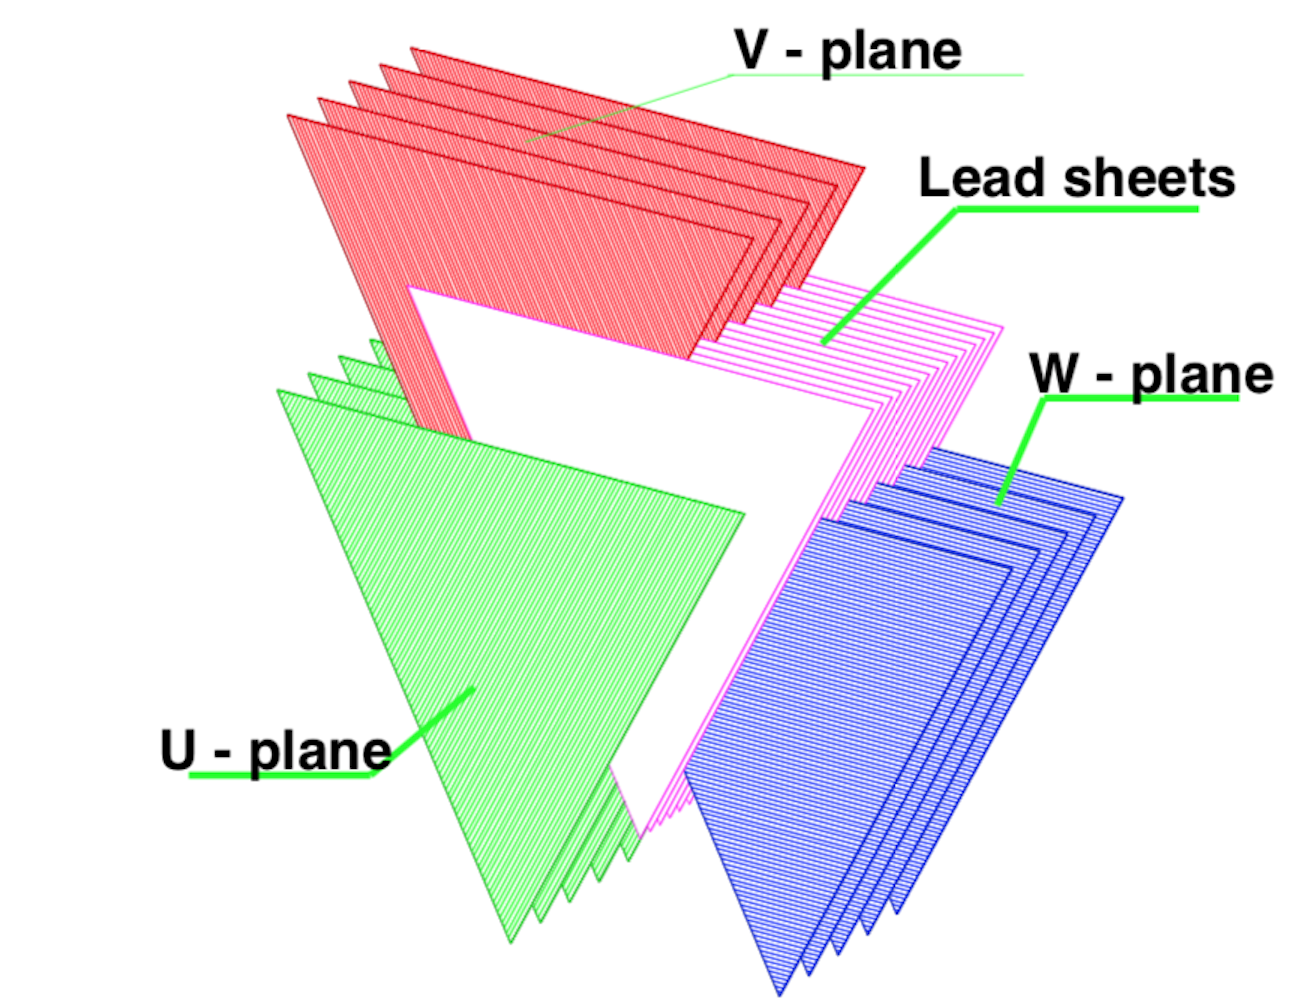
\includegraphics[width=3.in]{images/calorimeter_layers.png}
 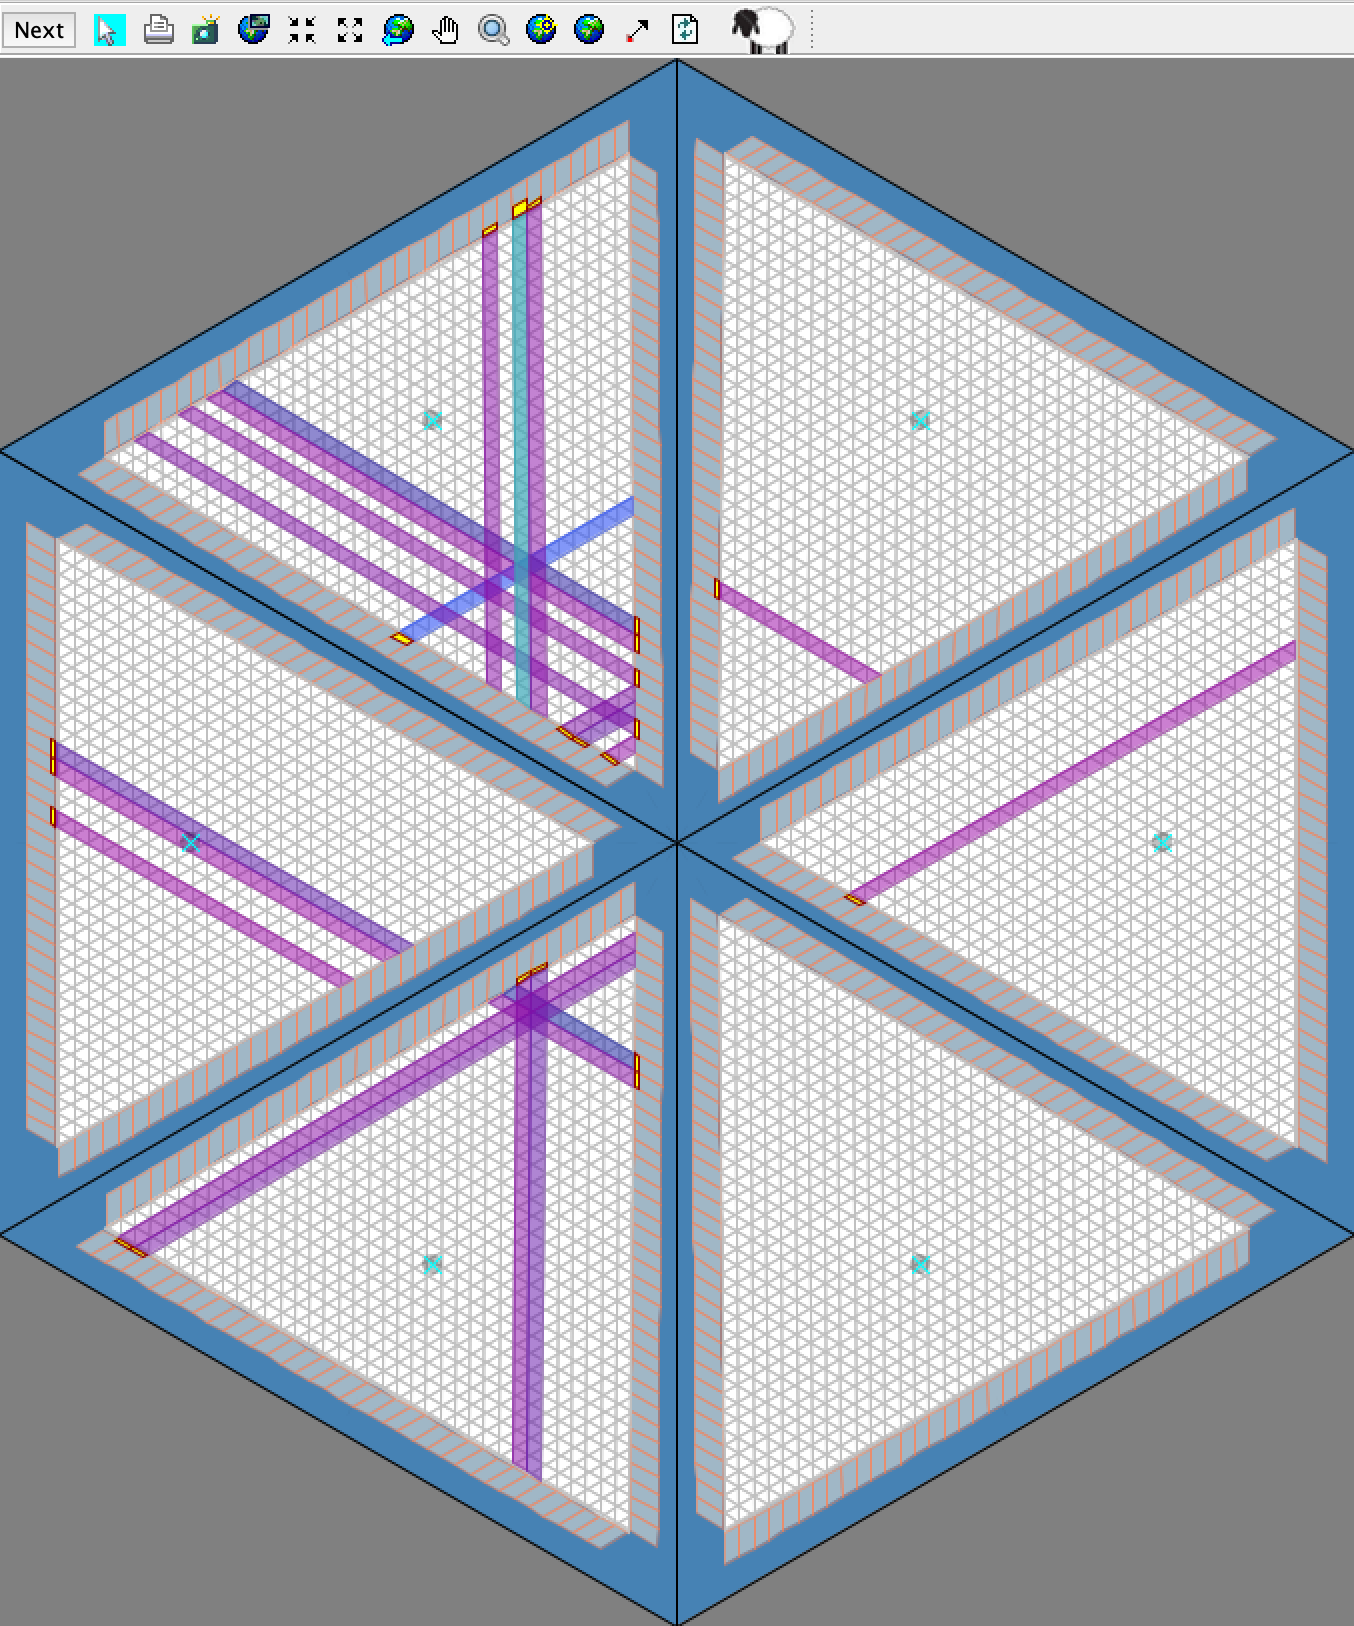
\includegraphics[width=2in]{images/ecal_view.png}
\caption { CLAS12 Electromagnetic Calorimeter structure description.}
 \label{clas12:ecal}
 \end{center}
\end{figure}

When particle enters the calorimeter it leaves signal in each of the layers (U,V and W), and is readout independently.
For each layer a cluster (called peak) is constructed by grouping adjacent hit strips and peaks from all three sides are combined into a cluster if they intersect in one point on the surface. A typical cluster is shown on Figure~\ref{clas12:ecal}.



\section{Acknowledgments}
This material is based upon work supported by the U.S. Department of Energy, Office of Science, Office of Nuclear Physics under contract DE-AC05-06OR23177, and NSF grant no. CCF-1439079 and the Richard T. Cheng Endowment. 
 
\newpage
\bibliography{references}
\bibliographystyle{ieeetr}

\end{document}
